\documentclass[border=0pt,tikz,10pt,varwidth=180mm]{standalone}
\usepackage{lmodern}
\usepackage{graphicx}
\usepackage{csvsimple}
\usepackage{tikzscale}
\usepackage{amsmath, esint}
\usepackage{amsfonts}
\usepackage{amssymb}
\usepackage{xcolor}
\setcounter{secnumdepth}{3}
%\usepackage[francais]{babel}
\usepackage[english]{babel}
% \usepackage{indentfirst}
\selectlanguage{english}
%\usepackage[utf8]{inputenc}
%\usepackage[T1]{fontenc}
%\usepackage{float}
\usepackage[colorlinks,bookmarks=false,linkcolor=blue,urlcolor=blue, citecolor=black]{hyperref}
\usepackage{placeins}
\usepackage{ulem}
\usepackage[squaren, cdot]{SIunits}
\usepackage{sistyle}
\usepackage{epstopdf}
%\usepackage{color}
\usepackage{pgf, tikz}
\usetikzlibrary{arrows,shapes,positioning}
\usetikzlibrary{datavisualization}
\usetikzlibrary{datavisualization.formats.functions}
\usetikzlibrary[
pgfplots.groupplots,
decorations,
decorations.pathmorphing,
decorations.pathreplacing,
decorations.text,
decorations.markings,
backgrounds,
chains,
calc,
automata,
arrows.meta,
intersections
]
\usepackage{scalefnt}
\usepackage{caption}
\usepackage{multirow}
\usepackage{wrapfig}
\usepackage{chemfig}
\usepackage{chemarr}
\usepackage{listings}
\usepackage{inconsolata}
\usepackage{color} 
\usepackage{pgfplots}
\usepgfplotslibrary{colormaps}
\usepackage{pgfplotstable}
\usepackage{svg}
\pgfplotsset{compat=newest}
\pgfplotstableset{col sep=comma}
\usepackage{cancel}
\usepackage{dirtytalk}
\usepackage{float}
\usepackage[export]{adjustbox}
\usepackage{pdfpages}

\definecolor{Gray}{rgb}{0.5, 0.5, 0.5}
\definecolor{Blue}{rgb}{0.0, 0.0, 1.0}
\definecolor{Olive}{rgb}{0.5, 0.5, 0.0}
\definecolor{Maroon}{rgb}{0.5, 0.0, 0.0}
\definecolor{applegreen}{rgb}{0.55, 0.71, 0.0}
\definecolor{ao}{rgb}{0.0, 0.5, 0.0}
\definecolor{bleudefrance}{rgb}{0.19, 0.55, 0.91}
\definecolor{actincolor}{HTML}{ffc311}
\definecolor{nuccolor}{HTML}{0600ff}
\definecolor{myosincolor}{HTML}{26a22b}
\definecolor{cyan}{rgb}{0.0, 1.0, 1.0}
\definecolor{RdPu1}{HTML}{feebe2}
\definecolor{RdPu2}{HTML}{f768a1}
\definecolor{RdPu3}{HTML}{7a0177}

\input{some_command}

\setlength{\parindent}{0pt}
\def\lx{0.5*\linewidth}

\begin{document}%
\begin{tikzpicture}%
\def\lx{0.5*\linewidth}%
\node[inner sep=0pt] (heat) at (-0.5,0) {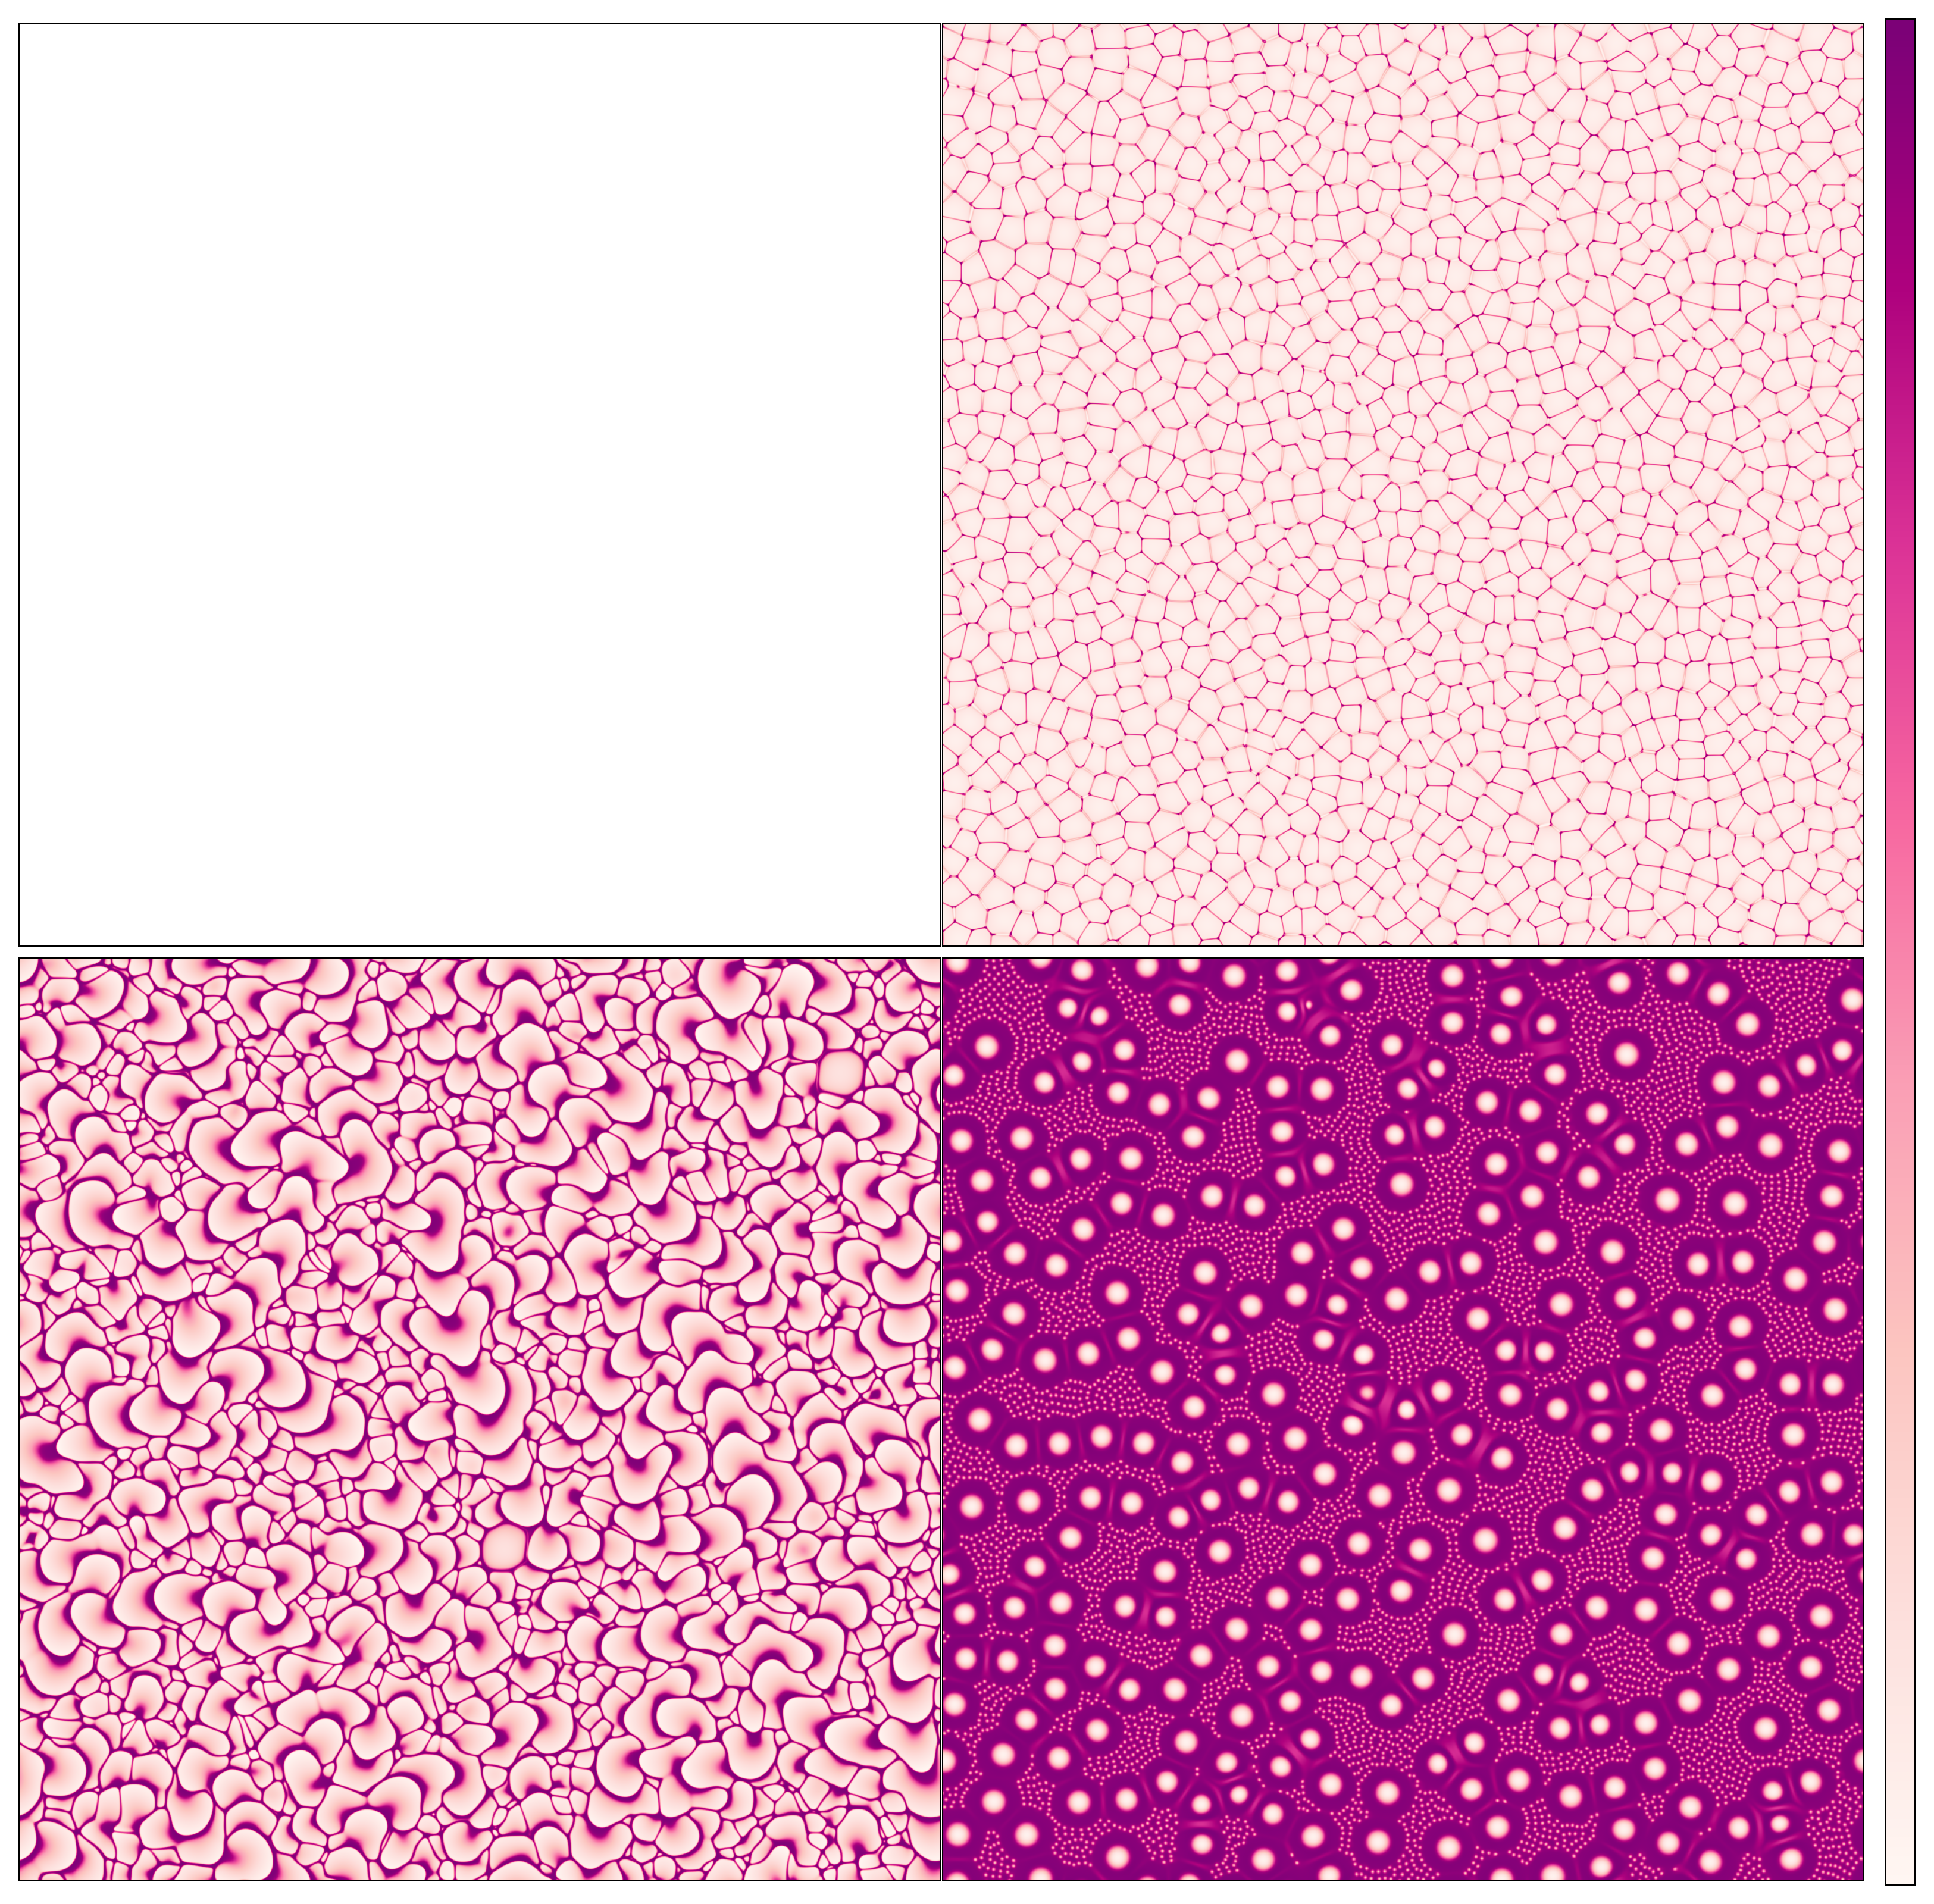
\includegraphics[width=0.9\linewidth]{phases_L50_3.png}};

\node at (0.89*\lx,-0.85*\lx) {$\rho_{min}$};
\node at (0.89*\lx,0.85*\lx) {$\rho_{max}$};
\node at (0.89*\lx,0) {$\rho$};

\node[text = black, rectangle, rounded corners=3pt, fill=white, opacity=0.85] at (-0.89*\lx, 0.82*\lx) {(a)};
\node[text = black, rectangle, rounded corners=3pt, fill=white, opacity=0.85] at (-0.02*\lx, 0.82*\lx) {(b)};
\node[text = black, rectangle, rounded corners=3pt, fill=white, opacity=0.85] at (-0.89*\lx, -0.05*\lx) {(c)};
\node[text = black, rectangle, rounded corners=3pt, fill=white, opacity=0.85] at (-0.02*\lx, -0.05*\lx) {(d)};

% Turnover
\fill[color=RdPu1] (-0.87*\lx,0.48*\lx) rectangle ++ (0.12*\lx,0.12*\lx);
\node[align=center] at (-0.81*\lx, 0.54*\lx) {$\rho<\rho_0$};
\draw[->, thick, >=stealth] (-0.75*\lx,0.54*\lx) -- ++(0.1*\lx,0);
\fill[color=RdPu2] (-0.65*\lx,0.48*\lx) rectangle ++ (0.12*\lx,0.12*\lx);
\node[align=center] at (-0.59*\lx, 0.54*\lx) {$\rho_0$};

\fill[color=RdPu3!70!RdPu2] (-0.87*\lx,0.62*\lx) rectangle ++ (0.12*\lx,0.12*\lx);
\node[align=center] at (-0.81*\lx, 0.68*\lx) {$\rho>\rho_0$};
\draw[->, thick, >=stealth] (-0.75*\lx,0.68*\lx) -- ++(0.1*\lx,0);
\fill[color=RdPu2] (-0.65*\lx,0.62*\lx) rectangle ++ (0.12*\lx,0.12*\lx);
\node[align=center] at (-0.59*\lx, 0.68*\lx) {$\rho_0$};

\node[align=center] at (-0.70*\lx,0.61*\lx) {$t\sim\tau$};
\node[align=center] at (-0.70*\lx,0.40*\lx) {\footnotesize renewal};

% Active stress
\fill[color=RdPu2] (-0.38*\lx,0.55*\lx) rectangle ++ (0.16*\lx,0.16*\lx);
\node[align=center] at (-0.3*\lx,0.63*\lx) {$\zeta_\rho\rho^3\Delta\mu$};
\draw[<-, color=ao, ultra thick, >=stealth] (-0.38*\lx,0.63*\lx)--(-0.45*\lx,0.63*\lx);
\draw[<-, color=ao, ultra thick, >=stealth] (-0.22*\lx,0.63*\lx)--(-0.15*\lx,0.63*\lx);
\draw[<-, color=ao, ultra thick, >=stealth] (-0.3*\lx,0.55*\lx)--(-0.3*\lx,0.48*\lx);
\draw[<-, color=ao, ultra thick, >=stealth] (-0.3*\lx,0.71*\lx)--(-0.3*\lx,0.78*\lx);
\node[align=center] at (-0.3*\lx,0.40*\lx) {\footnotesize active stress};

% Density-polarity Coupling
\node[align=center] at (-0.5*\lx,0.05*\lx) {\footnotesize density-polarity coupling ($p^2 \sim \rho/\rho_0$)};
\shade[left color=RdPu1, right color=RdPu3, middle color=RdPu2] (-0.8*\lx,0.1*\lx) rectangle ++ (0.6*\lx,0.2*\lx);
\draw[->, >=latex, ultra thick] (-0.7*\lx,0.17*\lx) -- (-0.7*\lx,0.23*\lx);
\draw[->, >=latex, ultra thick] (-0.5*\lx,0.15*\lx) -- (-0.5*\lx,0.25*\lx);
\draw[->, >=latex, ultra thick] (-0.3*\lx,0.13*\lx) -- (-0.3*\lx,0.27*\lx);
\end{tikzpicture}%
\end{document}
